\documentclass[a4paper,12pt]{article}
\usepackage[utf8]{inputenc}

\title{MA473 - Computational Finance \\ Pricing European, Barrier and American options with Spectral Collocation Methods}
\author{Abhinav R \\ Joel Raja Singh \\ Arav Garg}
\date{}

\usepackage{amsmath}
\usepackage{amsthm}
\usepackage{amsfonts}
\usepackage{mathtools}
\usepackage{enumitem}
\usepackage{graphicx}
\usepackage{caption}
\usepackage{subcaption}
\usepackage{needspace}

\begin{document}

\maketitle

\newcommand{\bsm}{\frac{\partial V(S, \tau)}{\partial \tau} = rS\frac{\partial V(S, \tau)}{\partial S} + \frac{1}{2}\sigma^2\frac{\partial^2 V(S, \tau)}{\partial S^2} - rV(S, \tau)}
\newcommand{\bsmg}{\frac{\partial V(S, \tau)}{\partial \tau} = rS\frac{\partial V(S, \tau)}{\partial S} + \frac{1}{2}\sigma^2\frac{\partial^2 V(S, \tau)}{\partial S^2} - rV(S, \tau) + g(V(S, \tau))}
\newcommand{\R}{\mathbb{R}}
\newcommand{\norm}[1]{{\left \lVert #1 \right \rVert}_2}
\newcommand{\floor}[1]{\lfloor #1 \rfloor}
\newcommand{\er}{\operatorname{Error}_{m,N}(S)}

\section{Introduction}

In this project, we make an independent implementation and reproduce the results from \cite{col}, where the authors present a scheme based on spectral collocation to solve the partial differential equations that arise while pricing standard options in the Black-Scholes framework. 

\section{Preliminaries}

In this section, we briefly describe the Black-Scholes framework and the PDEs to be solved for pricing relevant options under the same. We assume that the price of the underlying asset ($S$) evolves according to the SDE:
\begin{equation}
    dS(t) = \mu S(t)dt + \sigma S(t) dW(t)
\end{equation}
where $\mu$ and $\sigma$ are the (constant) drift and volatility and $W(t)$ is the standard Wiener process. For the sake of simplicity, we assume that the underlying asset does not pay dividends. 

Using this setup along with the no-arbitrage principle, we may obtain pricing formulas for several options as solutions to the Black-Scholes PDE with different boundary and initial conditions. For any option, let $T$ be its time of maturity and $V(S, \tau)$ be its value at time $0 \leq t \leq T$, where $\tau = T - t$. We state the IBVPs for $V(S, \tau)$ below: (In all the equations below, $E$ is the strike price of the option and $r$ is the risk-free rate.)
\begin{enumerate}
    \item \textbf{European call:} For $0 < \tau \leq T$ and $S \geq 0$, $V$ satisfies, 
    \begin{equation}
        \bsm
    \end{equation}
    with initial condition,
    \begin{equation*}
        V(S,0) = \max(S - E, 0)
    \end{equation*}
    and boundary conditions,
    \begin{equation*}
        \begin{split}
            V(0, \tau) &= 0\\
            \lim_{S \to \infty} V(S, \tau) &= S - E\exp\left(-r\tau\right)\\
        \end{split}
    \end{equation*}
    
    \item \textbf{Up and Out Barrier Call:} For $0 < \tau \leq T$ and $0 \leq S < B$, where $B$ is the barrier, $V$ satisfies,
    \begin{equation}
        \bsm
    \end{equation}
    with initial condition,
    \begin{equation*}
        V(S,0) = \max(S - E, 0)
    \end{equation*}
    and boundary conditions,
    \begin{equation*}
        \begin{split}
            V(0, \tau) &= 0\\
            V(B, \tau) &= 0\\
        \end{split}
    \end{equation*}
    
    Both the European call and Up and Out barrier call options have closed form solutions (refer \cite{stoch}).
    
    \item \textbf{American Put:} For $0 < \tau \leq T$, $V$ satisfies the free-boundary PDE,
    \begin{equation}
        \bsm \quad S > B(\tau)
    \end{equation}
    \begin{equation*}
        V(S, \tau) = E - S \quad 0 \leq S \leq B(\tau)
    \end{equation*}
    with the smooth pasting condition,
    \begin{equation*}
        \frac{\partial V(B(\tau), \tau)}{\partial S} = -1 
    \end{equation*}
    initial condition,
    \begin{equation*}
        V(S, 0) = \max(E-S, 0)
    \end{equation*}
    and finally boundary condition,
    \begin{equation*}
        \lim_{S \to \infty} V(S, \tau) = 0
    \end{equation*}
    Where $B(\tau)$ is the free-boundary or the early-exercise curve. Also, to avoid arbitrage, $V$ must also satisfy,
    \begin{equation*}
        V(S, \tau) \geq \max(E - S,0) \quad S \geq 0, 0 \leq \tau \leq T
    \end{equation*}
    
    To resolve the complications arising from the free-boundary, we replace the original PDE with a non-linear PDE by adding a penalty term. The reformulated PDE is as follows:
    \begin{equation}
        \bsm + \frac{\epsilon C}{V(S, \tau) + \epsilon - E + S} \quad S\geq0
    \end{equation}
    with initial condition,
    \begin{equation*}
        V(S, 0) = \max(E-S,0)
    \end{equation*}
    and boundary conditions,
    \begin{equation*}
        \begin{split}
            V(0,\tau) &= E\\
            \lim_{S \to \infty}V(S, \tau) &= 0\\
        \end{split}
    \end{equation*}
    
    To this end, we introduce the function $g$ such that for the American put,
    \begin{equation}
        g(V(S,\tau)) = \frac{\epsilon C}{V(S, \tau) + \epsilon - E + S}
    \end{equation}
    and for the other two options $g(V(S,\tau)) = 0$, so that we may write the PDE for all three options together as,
    \begin{equation}
        \bsmg
    \end{equation}
    Thus, for every option under consideration, we solve equation (7) with initial conditions $\psi(S)$ and boundary conditions $\phi_1(\tau)$ at $S = 0$ and $\phi_2(\tau)$ at $S = \infty$, where each function takes the form corresponding to the option as presented above.
\end{enumerate}

\section{Chebyshev Polynomials and Interpolation}

Let $\{T_n(x)\}_{n=0}^\infty$ be the class of Chebyshev polynomials. Consider the extreme points of these polynomials (Chebyshev-Gauss-Lobatto, or CGL points) given by,
\begin{equation}
    \xi_k = \cos \left( \frac{k\pi}{N} \right) \quad k = 0, \dots, N
\end{equation}

We define the Lagrange polynomials with CGL points as:
\begin{equation}
    L_j(x) = \prod_{i=0, i \neq j}^N \frac{x - x_i}{\xi_j - \xi_i} \quad j = 0, \dots, N
\end{equation}

With these polynomials, we may interpolate a given function $u \in L^2(\R^2)$ with domain $[-1,1] \times [0,T]$ as,
\begin{equation}
    p(u(x,t)) = \sum_{j = 0}^N u(\xi_j , t) L_j(x)
\end{equation}
We also have the approximation for $\frac{\partial u}{\partial x}$ over the CGL points as,
\begin{equation}
    p(u_x(\xi_k,t)) = \sum_{j = 0}^N u(\xi_j , t) D_{j,k}^{(1)}
\end{equation}
where $D_{j,k}^{(1)} = \frac{\partial L_j(x)}{\partial x} |_{x = \xi_k}$ and the matrix $D^{(1)} = [[D_{j,k}^{(1)}]]$ is called the matrix of the derivative of the first kind Chebyshev polynomials. Similarly we have the approximation for $\frac{\partial^2 u}{\partial x^2}$ as,
\begin{equation}
    p(u_{xx}(\xi_k,t)) = \sum_{j = 0}^N u(\xi_j , t) D_{j,k}^{(2)}
\end{equation}
where $D_{j,k}^{(2)} = \frac{\partial^2 L_j(x)}{\partial x^2} |_{x = \xi_k}$ and $D^{(2)}$ is defined analogously to $D^{(1)}$.

We use (10)-(12) along with a domain decomposition of the domain of $S$ to numerically solve the PDE (7).

\section{Solving the PDEs Numerically}

For all of the above problems, we first truncate the infinite domain $[0, \infty]$ of $S$ to $\Omega = [0,S_{max}]$ where for each option, we choose $S_{max}$ in the way described in \cite{col}, Section 6.

Further, we decompose the domain $\Omega$ into $m$ subdomains of the form $\Omega_i = [S_{i-1}, S_i]$ for $i = 1, \dots, m$ such that $S_0 = 0 < S_1 \dots < S_m = S_{max}$. Clearly, $\bigcup_{i=1}^m \Omega_i = \Omega$. Thus, we would have to solve the BS PDE for each domain,

\begin{equation}
    \frac{\partial V_i(S, \tau)}{\partial \tau} = rS\frac{\partial V_i(S, \tau)}{\partial S} + \frac{1}{2}\sigma^2\frac{\partial^2 V_i(S, \tau)}{\partial S^2} - rV_i(S, \tau) + g(V_i(S,\tau)) \quad S \in [S_{i-1}, S_i]
\end{equation}
for $i = 1, \dots, m$.

Now, we transform each domain $\Omega_i$ to $[-1,1]$ via the transformation,
\begin{equation}
    X_i(x) = S = \frac{S_i - S_{i-1}}{2}x + \frac{S_i + S_{i-1}}{2}
\end{equation}
Applying this transformation and setting $V_i(S, \tau) = u_i(x, \tau)$ reduces (13) to the set of equations,

\begin{equation}
    \frac{\partial u_i(x, \tau)}{\partial \tau} = R_i^{(1)}(x)\frac{\partial u_i(x, \tau)}{\partial x} + R_i^{(2)}(x)\frac{\partial^2 u_i(x, \tau)}{\partial x^2} - ru_i(x, \tau) + g(u_i(x,\tau)) \quad x \in [-1,1]
\end{equation}
where,
\begin{equation}
    \begin{split}
        R_i^{(1)}(x) &= rX_i(x) \frac{2}{S_i - S_{i-1}}\\
        R_i^{(2)}(x) &= \frac{1}{2} \sigma^2 \left(X_i(x) \frac{2}{S_i - S_{i-1}}\right)^2\\
    \end{split}
\end{equation}
with initial and boundary conditions,
\begin{equation}
    \begin{split}
        u_i(x,0) &= \psi(X_i(x)) \quad i = 1, \dots, m\\
        u_1(-1, \tau) &= \phi_1(\tau)\\
        u_m(1, \tau) &= \phi_2(\tau)\\
    \end{split}
\end{equation}
Additionally, we impose the smoothness conditions,
\begin{equation}
    \begin{split}
        u_i(1, \tau) &= u_{i+1}(-1,\tau) \\
        \frac{\partial u_i (x,\tau)}{\partial x}|_{x = 1} &= \frac{\partial u_{i+1} (x,\tau)}{\partial x}|_{x = -1}\\
    \end{split}
\end{equation}
for $i = 1, \dots, m-1$.

Combining (18) with the interpolation in (11) gives us the following form for $du_i(\tau) := u_i(1, \tau)$,
\begin{equation}
    du_i(\tau) = \frac{1}{D_{0,0}^{(1)} - D_{N,N}^{(1)}} \left( \sum_{j=0}^{N-1} u_{i+1}(\xi_j, \tau)D_{j,N}^{(1)} - \sum_{j=1}^{N} u_{i}(\xi_j, \tau)D_{j,0}^{(1)} \right)
\end{equation}

Now, multiplying (15) by the Dirac delta $\delta(x - \xi_j)$ and integrating for $j = 0, \dots, N$ gives us the system of ODEs in $\tau$,

\begin{equation}
    \frac{\partial u_i(\xi_j, \tau)}{\partial \tau} = R_i^{(1)}(\xi_j)\frac{\partial u_i(x, \tau)}{\partial x}|_{x = \xi_j} + R_i^{(2)}(\xi_j)\frac{\partial^2 u_i(x, \tau)}{\partial x^2}|_{x = \xi_j} - ru_i(\xi_j, \tau) + g(u_i(\xi_j,\tau))
\end{equation}
for $i = 1, \dots, m$ and $j = 0, \dots N$.

Now, for the partial derivatives of $x$, we may use the interpolation formulas from (11) and (12) to further simplify this system of ODEs. Detailed calculations are presented in \cite{col} and the precise system of ODEs is obtained in equations (4.21) - (4.24) in \cite{col}. Succinctly, it is represented as,

\begin{equation}
    \begin{split}
        \frac{dU(\tau)}{d\tau} &= F(\tau, U(\tau))\\
        U(0) &= U_0\\
    \end{split}
\end{equation}
where $U(\tau) \in \R^{mN - 1}$ (as it doesn't include boundary terms) and $F$ takes the form as in \cite{col}, (4.23).

To solve the IVP in (21), we adopt a predictor-corrector approach where the predictor step follows the Euler method and the corrector step follows the Trapezoidal method. Also, we use a variable step size approach for fast convergence. The key idea behind variable step size is to choose the next step optimally so as to reduce the chance of unstable numerical behaviour. Concretely, the scheme is summarized as follows:

\begin{equation}
    \begin{split}
        U_{n+1}^{(1)} &= U_n + h_n F(\tau_n, U_n)\\
        U_{n+1}^{(\mu)} &= U_n + \frac{h_n}{2}\left( F(\tau_n, U_n) + F(\tau_{n+1}, U_{n+1}^{(1)}) \right)
    \end{split}
\end{equation}
Also, we define,
\begin{equation}
    \operatorname{Er}_{n+1} = \norm{U_{n+1}^{(\mu)} - U_{n+1}^{(1)}}
\end{equation}
where Tol is a predefined tolerance level for the scheme. The step size evolves as follows:
\begin{equation}
    \begin{split}
        h_{n+1}^* &= h_n\left( \frac{\alpha \operatorname{Tol}}{\operatorname{Er}_{n+1}} \right)^{1/(p+1)}\\
        h_{n+1} &= \min(h_{n+1}^*, 2)\\
    \end{split}
\end{equation}
In total, we repeat (22) until $\operatorname{Er}_{n+1} < \operatorname{Tol}$, where in every repetition, we halve $h_n$ (We denote the initial step size chosen by the user as $h_0$). Each such repetition corresponds to a "rejected step". Once $\operatorname{Er}_{n+1} < \operatorname{Tol}$ is achieved, we "accept" the step and set the next step size as per equations in (24) where we choose $\alpha = 0.5$ and $p$ is the order of the method (here, $p = 2$).

In the case of the American put, we must also add an additional step before after each computation in (22) to maintain $V(S, \tau) \geq E - S$ as follows:

\begin{equation}
    U_{n+1}^{(j)} = \max(U_{n+1}^{(j)}, U_0)
\end{equation}
where $\max$ is the component-wise maximum. We now proceed to examine the results obtained from implementing these schemes.

\section{Numerical Experiments}

In this section, we present the results of the actual implementation of the methodology explained in the previous sections. The MATLAB programs \texttt{eur\_call.m} , \texttt{b\_call.m} and \texttt{a\_put.m} can be used to obtain all the results presented for the European Call, Up and Out Barrier call and American put respectively. (The \texttt{README.txt} file presents short descriptions of each program.)

As mentioned in \cite{col}, for the European call and American put, we always take,
\begin{equation}
    S_{max} = \frac{mE}{\floor{\frac{m}{2}}}
\end{equation}
This is so that we encounter minimal error from the truncation of the original half-infinite strip and also to make sure that $E$ is one of the points $\{S_i\}$. 
Similarly, for the Barrier call $S_{max} = B$. So, given $B$ and $E$, we make sure that,
\begin{equation}
    E = \frac{k}{m}B
\end{equation}
for some $k = 1, \dots, m$. 

Also, for all the results we express the error as the maximum error at $\tau = T$ (or $t = 0$). That is,
\begin{equation}
    \er = \max_S \lvert V(S,T) - \hat{V}(S,T) \rvert
\end{equation}
where for the European and Barrier call, $\hat{V}$ is the actual solution and for the American put, it is the solution obtained via the binomial pricing algorithm (as no closed form solution is known to the free-boundary PDE) with 1000 time steps between $t = 0$ and $t = T$ (i.e, height of the tree = 1000).

(All the computations were done over an instance of MATLAB Online R2021a. Also, note that the time readings are much higher than those in \cite{col} because in our MATLAB programs, we store the solution for all time steps whereas it would reduce much cost if we store only $V(S, T)$.)

\subsection{European and Barrier Call}
We choose all the parameter values exactly as in \cite{col}. That is, we choose the following parameter values for the European call: $\sigma = 0.2$, $r = 0.05$, $T = 0.5$, $E = 10$. The parameters for the Barrier call are: $\sigma = 0.2$, $r = 0.05$, $T = 0.5$, $E = 100$, $B = 120$.

Table 1 details the observations for fixed $N = 10$ and varying $m$, Tol  and $h_0$. The column "Ratio" expresses the convergence ratio as the ratio between two consecutive entries (coarser / finer discretization) in the Error column. Accepted Steps is the total number of accepted steps to reach $\tau = T$ in the variable step size approach.

Table 2 details the observations for fixed $m = 12$ and different values of $N$. 

Table 3 shows the error and accepted steps in the case of the Up and Out Barrier Call for various values of $m$ and $N$. 

Finally, Table 4 and 5 compare the variable step size method against the constant step size method in the European Call case.

Figure 1 shows the plot of $\er$ for $m = N = 10$, Tol = $10^{-6}$ and $h_0 = 10^{-3}$ (with Accepted steps = 1958). 

Figure 2 and 3 show the plot of $V(S,T)$ vs. $\hat{V}(S, T)$ for the European and Barrier call respectively. For the European case, $m = 5$, $N = 8$, Tol = $10^{-5}$ and $h_0 = 10^{-2}$ (Accepted steps = 427). For the Barrier case, $m = 6$, $N = 8$, Tol = $10^{-3}$ and $h_0 = 10^{-2}$ (Accepted steps = 570).  

\subsection{American Put}
We use the following values for parameters : $\sigma = 0.3$, $r = 0.1$, $T = 1$, $E = 1$. Additionally for the penalty $g$, we use parameters $C = rE$ and $\epsilon = 10^{-4}$. We summarize our observations in Tables 6-10.

Table 6 shows observations for $N = 8$ and different values of $m$.

Table 7 shows observations for $m = 16$ and different values of $N$.

Table 8 shows the effect of decreasing $\epsilon$ in the penalty method.

Table 9 and 10 compare the variable step size and constant step size approaches.

Figure 4 shows computed $V(S,T)$ for $m = 7$, $N = 11$, Tol = $10^{-6}$, $h_0 = 10^{-4}$ (Accepted steps = 3188) against the maturity payoff.

Finally, Figure 5 shows the plot of $V(S,T)$ vs. $\hat{V}(S, T)$, $m = 7$, $N = 8$, Tol = $10^{-5}$ and $h_0 = 10^{-2}$ (Accepted steps = 789).


 \begin{table}
 \begin{center}
 \caption{European call, $N = 10$}
 \begin{tabular}{||c c c c c c c||} 
 \hline
 $m$ & $\er$ & Ratio & Tol & $h_0$ & Accepted Steps & cpu t (s) \\ [0.5ex] 
 \hline\hline
 4 & $3.30 \times 10^{-4}$ & - & $10^{-3}$ & $10^{-1}$ & 159 & 1.05\\ 
 \hline
 7 & $1.99 \times 10^{-6}$ & 165.83 & $10^{-5}$ & $10^{-3}$ & 675 &  5.2\\
 \hline
 12 & $6.91 \times 10^{-8}$ & 28.79 & $10^{-7}$ & $10^{-4}$ & 6199 & 74.91 \\
 \hline
 15 & $8.77 \times 10^{-9}$ & 7.88 & $10^{-8}$ & $10^{-4}$ & 20237 & 368.07 \\
 \hline
\end{tabular}
\end{center}
\end{table}



 \begin{table}
 \caption{European call, $m = 12$}
 \begin{center}
 \begin{tabular}{||c c c c c c c||} 
 \hline
 $N$ & $\er$ & Ratio & Tol & $h_0$ & Accepted Steps & cpu t (s) \\ [0.5ex] 
 \hline\hline
 5 & $3.00 \times 10^{-3}$ & - & $10^{-2}$ & $10^{-2}$ & 101 & 0.87\\ 
 \hline
 7 & $2.51 \times 10^{-5}$ & 119.52 & $10^{-4}$ & $10^{-2}$ & 391 & 2.82\\
 \hline
 9 & $1.76 \times 10^{-7}$ & 142.61 & $10^{-6}$ & $10^{-3}$ & 1944 & 18.53 \\
 \hline
 11 & $6.91 \times 10^{-8}$ & 2.55 & $10^{-7}$ & $10^{-4}$ & 6414 & 104.99 \\
 \hline
\end{tabular}
\end{center}
\end{table}


 \begin{table}
 \caption{Barrier call}
 \begin{center}
 \begin{tabular}{||c c c c c c c c||} 
 \hline
 $N$ & $m$ & $\er$ & Ratio & Tol & $h_0$ & Accepted Steps & cpu t (s) \\ [0.5ex] 
 \hline\hline
 7 & 6 & $3.23 \times 10^{-4}$ & - & $10^{-3}$ & $10^{-2}$ & 521 & 2.03\\ 
 \hline
 7 & 12 & $1.94 \times 10^{-5}$ & 16.65 &$10^{-4}$ & $10^{-3}$ & 2155 & 14.46 \\
 \hline
 7 & 24 & $1.21 \times 10^{-5}$ & 1.60 &$10^{-4}$ & $10^{-4}$ & 3261 & 45.59 \\
 \hline
 9 & 6 & $8.30 \times 10^{-6}$ & - &$10^{-4}$ & $10^{-4}$ & 1919 & 9.86\\
 \hline
 9 & 12 & $3.89 \times 10^{-7}$ & 21.34 &$10^{-5}$ & $10^{-4}$ & 7824 & 80.49\\
\hline
 9 & 24 & $2.79 \times 10^{-8}$ & 13.94 &$10^{-6}$ & $10^{-4}$ & 31446 & $1.14 \times 10^{3}$\\
 \hline
\end{tabular}
\end{center}
\end{table}



 \begin{table}
 \caption{European call, variable step size}
\begin{center}
 \begin{tabular}{||c c c c c c||} 
 \hline
 $m, N$ & $\er$ & Tol & $h_0$ & Accepted Steps & cpu t (s) \\ [0.5ex] 
 \hline\hline
 4,7 &  $3.50 \times 10^{-3}$ & $10^{-2}$ & $10^{-2}$ & 37 & 0.46\\ 
 \hline
 7,11 & $2.59 \times 10^{-6}$ & $10^{-5}$ & $10^{-3}$ & 866 & 8.49 \\
 \hline
 9,12 & $1.55 \times 10^{-8}$ & $10^{-7}$ & $10^{-4}$ & 6057 & 93.52 \\
 \hline
\end{tabular}
\end{center}
\end{table}

 \begin{table}
\begin{center}
 \caption{European call, constant step size}
 \begin{tabular}{||c c c c||} 
 \hline
 $m, N$ & $\er$ & Steps & cpu t (s) \\ [0.5ex] 
 \hline\hline
 4,7 &  $3.60 \times 10^{-3}$ & 500  & 1.65\\ 
 \hline
 7,11 & $2.53 \times 10^{-6}$ & 5000 & 52.71 \\
 \hline
 9,12 & $1.83 \times 10^{-8}$ & 10000 & 149.83 \\
 \hline
\end{tabular}
\end{center}
\end{table}


 \begin{table}
 \caption{American put, $N = 8$}
\begin{center}
 \begin{tabular}{||c c c c c c ||} 
 \hline
 $m$ & $\er$  & Tol & $h_0$ & Accepted Steps & cpu t (s) \\ [0.5ex] 
 \hline\hline
 3 & $8.34 \times 10^{-2}$  & $10^{-2}$ & $10^{-2}$ & 74 & 0.47\\ 
 \hline
 4 & $4.70 \times 10^{-2}$  & $10^{-3}$ & $10^{-2}$ & 164 & 0.84 \\
 \hline
 5 & $4.68 \times 10^{-2}$  & $10^{-3}$ & $10^{-3}$ & 280 & 1.53 \\
 \hline
 7 & $1.20 \times 10^{-2}$  & $10^{-4}$ & $10^{-3}$ & 677 & 3.46 \\
 \hline
 8 & $7.58 \times 10^{-4}$  & $10^{-5}$ & $10^{-3}$ & 1118 & 6.43 \\
 \hline
\end{tabular}
\end{center}
\end{table}


 \begin{table}
 \caption{American put, $m = 16$}
\begin{center}
 \begin{tabular}{||c c c c c c||} 
 \hline
 $N$ & $\er$  & Tol & $h_0$ & Accepted Steps & cpu t (s) \\ [0.5ex] 
 \hline\hline
 2 & $3.29 \times 10^{-2}$  & $10^{-3}$ & $10^{-2}$ & 38 & 0.45\\ 
 \hline
 4 & $5.80 \times 10^{-3}$  & $10^{-4}$ & $10^{-2}$ & 378 & 1.84 \\
 \hline
 6 & $5.97 \times 10^{-4}$  & $10^{-6}$ & $10^{-3}$ & 1834 & 12.76\\
 \hline
 7 & $7.65 \times 10^{-4}$  & $10^{-5}$ & $10^{-3}$ & 2750 & 24.40\\
 \hline
 10 & $5.34 \times 10^{-4}$  & $10^{-7}$ & $10^{-5}$ & 12018 & 213.53 \\
 \hline
\end{tabular}
\end{center}
\end{table}


 \begin{table}
\begin{center}
 \caption{American put, $m = 8$, $N = 9$, $h_0 = 10^{-3}$, Tol = $10^{-5}$}
 \begin{tabular}{||c c c c||} 
 \hline
 $\epsilon$ & $\er$ & Accepted Steps & cpu t (s) \\ [0.5ex] 
 \hline\hline
 $10^{-1}$ &  $4.01 \times 10^{-2}$ & 1897 & 12.61\\ 
 \hline
 $10^{-2}$ & $1.29 \times 10^{-2}$ & 1899 & 13.21 \\
 \hline
 $10^{-3}$ & $2.70 \times 10^{-3}$ & 1792 & 12.29 \\
 \hline
 $10^{-4}$ & $5.34 \times 10^{-4}$ & 1719 & 12.01 \\
 \hline
 $10^{-4.2}$ & $5.33 \times 10^{-4}$ & 1717 & 11.62 \\
 \hline
\end{tabular}
\end{center}
\end{table}

\begin{table}
 \caption{American put, variable step size}
\begin{center}
 \begin{tabular}{||c c c c c c||} 
 \hline
 $m, N$ & $\er$ & Tol & $h_0$ & Accepted Steps & cpu t (s) \\ [0.5ex] 
 \hline\hline
 6,8 &  $1.20 \times 10^{-2}$ & $10^{-5}$ & $10^{-1}$ & 639 & 3.03\\ 
 \hline
 8,9 & $5.34 \times 10^{-4}$ & $10^{-6}$ & $10^{-6}$ & 2078 & 14.29 \\
 \hline
\end{tabular}
\end{center}
\end{table}

 \begin{table}
\begin{center}
 \caption{American put, constant step size}
 \begin{tabular}{||c c c c||} 
 \hline
 $m, N$ & $\er$ & Steps & cpu t (s) \\ [0.5ex] 
 \hline\hline
 6,8 &  $1.20 \times 10^{-2}$ & 5000 & 22.25\\ 
 \hline
 8,9 & $5.34 \times 10^{-4}$ & 10000 & 75.59 \\
 \hline
\end{tabular}
\end{center}
\end{table}

\newpage

\section{Conclusion}

In this project, we used a spectral collocation scheme along with domain decomposition to obtain a system of ODEs in the time-direction to solve the BS PDE. We can observe from the tables and figures that the method efficiently solves the PDE and outperforms the constant step size approach as well.


\begin{figure}[p]
        \centering
        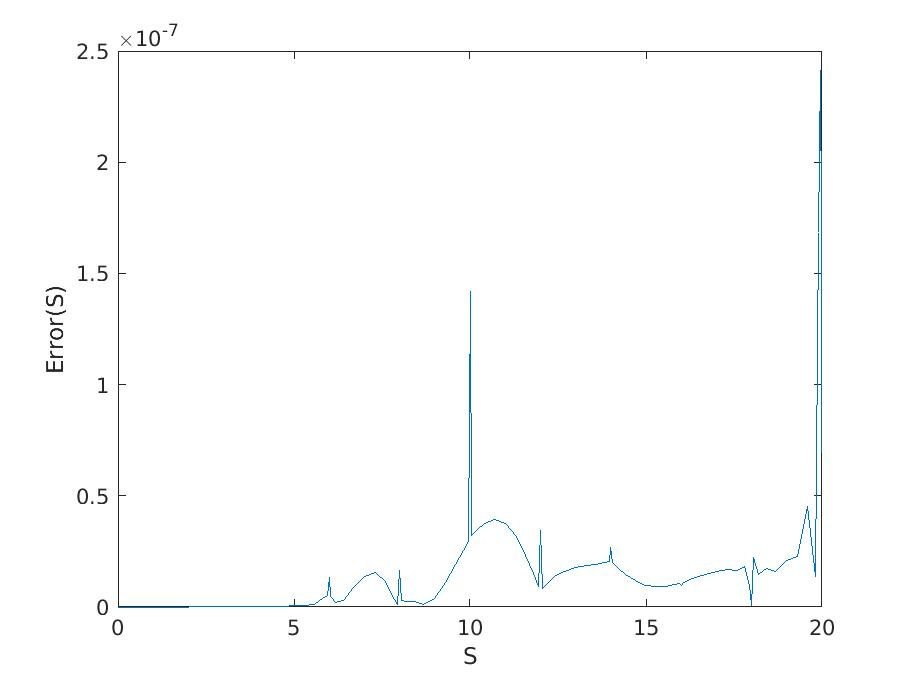
\includegraphics[width = \linewidth]{err_eur.jpg}
        \caption{Plot of Error(S), $m=N=10$, European Call}
        \label{fig:q}
\end{figure}

\begin{figure}[p]
        \centering
        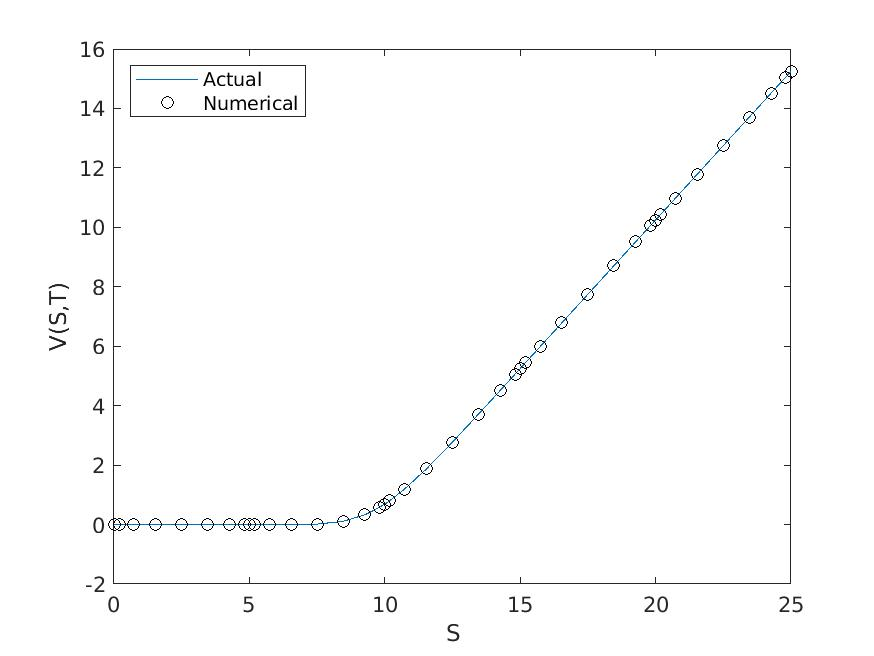
\includegraphics[width = \linewidth]{eur_vs (1).jpg}
        \caption{$V(S,T)$ vs $\hat{V}(S,T)$, $m=5$, $N=8$, European Call}
        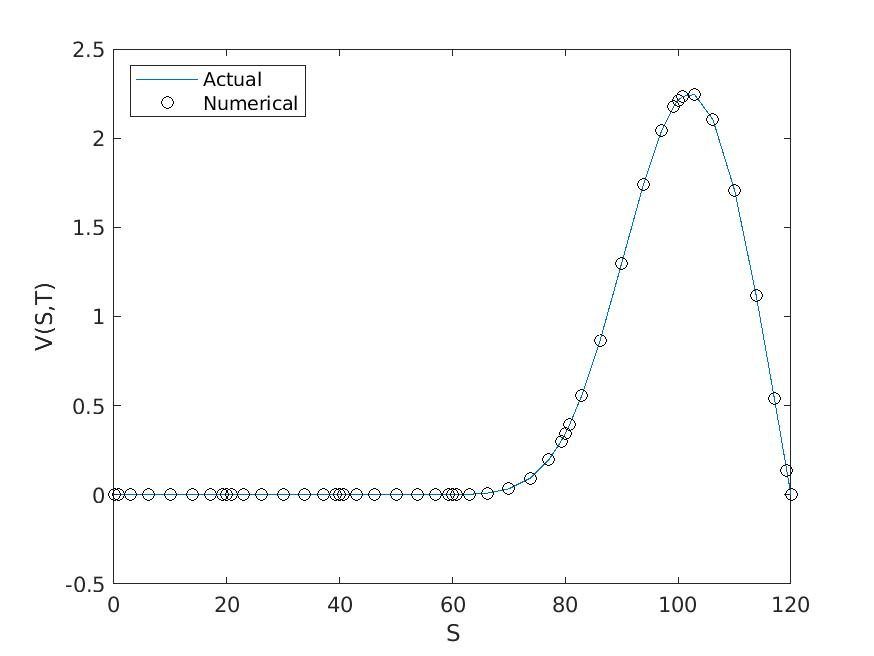
\includegraphics[width = \linewidth]{b_vs.jpg}
        \caption{$V(S,T)$ vs $\hat{V}(S,T)$, $m=6$, $N=8$, Barrier Call}
\end{figure}

\begin{figure}[p]
        \centering
        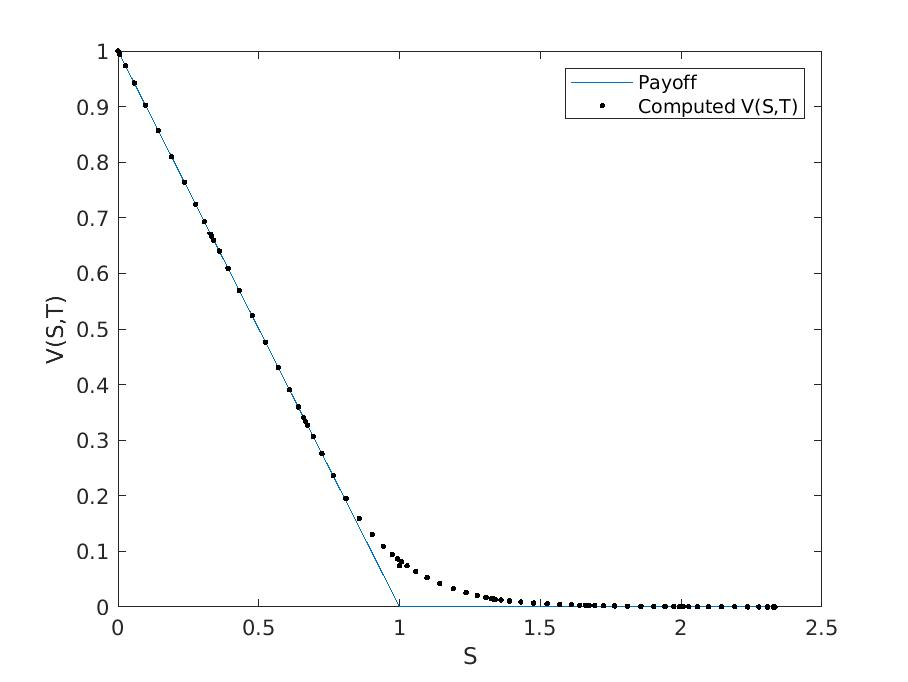
\includegraphics[width = \linewidth]{vst_a.jpg}
        \caption{$V(S,T)$ vs Payoff, $m=7$, $N=11$, American Put}
        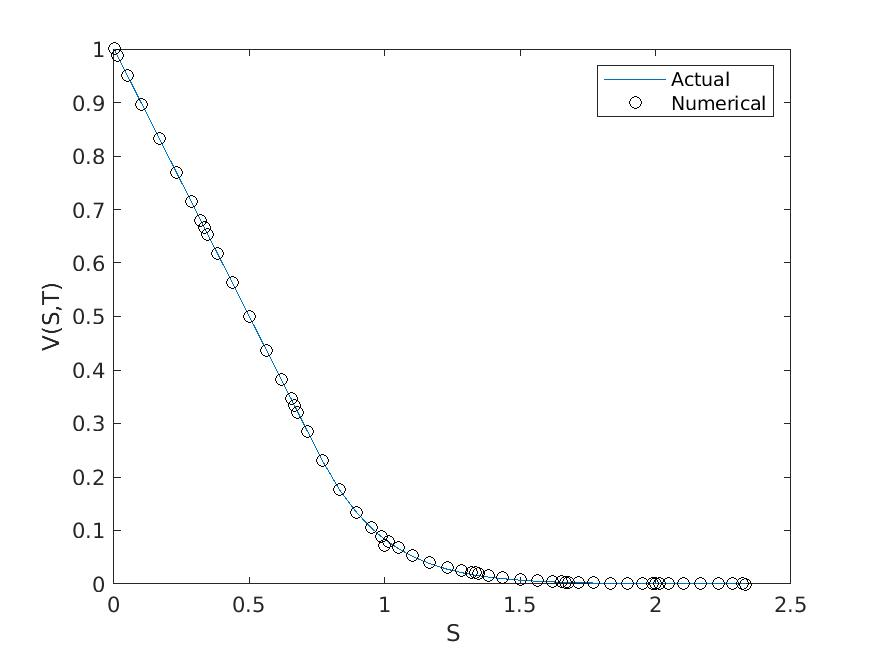
\includegraphics[width = \linewidth]{a_vs.jpg}
        \caption{$V(S,T)$ vs $\hat{V}(S,T)$, $m=7$, $N=8$, American Put}
\end{figure}

\newpage
    \bibliographystyle{plain}
    \bibliography{bib.bib}

\end{document}
